\section{From penalized least squares to a smoothness coordinate}
\label{sec:expanded-theory}
Let $y=(y_1,\dots,y_n)^\top$ denote equally spaced observations.
For $1\leq d<n$, define the $d$th forward-difference operator
$D_d\in\mathbb R^{(n-d)\times n}$, so $D_1\tau$ contains consecutive
increments and $D_2\tau$ contains consecutive differences of increments.
The order is not itself a smoothness magnitude: it defines which
local changes are penalized. With a reference difference mean
$\mu$, our fitted trend is
\begin{equation}
\widehat{\tau}_{\lambda,\mu}
=\arg\min_\tau\bigl\{\|y-\tau\|_2^2+
  \lambda\|D_d\tau-\mu\mathbf1\|_2^2\bigr\},\quad
  \lambda\ge0 .
\label{eq:expanded-pls}
\end{equation}
The normal equations give
\begin{equation}
(I+\lambda Q_d)\widehat\tau_{\lambda,\mu}
=y+\lambda\mu D_d^\top\mathbf1,\qquad Q_d=D_d^\top D_d.
\label{eq:expanded-normal}
\end{equation}
Since the objective is strictly convex for every finite
$\lambda\ge0$, the solution is unique.

\subsection{Null space, order and reference differences}
The rows of $D_d$ are linearly independent, and hence
$\operatorname{rank}(Q_d)=n-d$. Its null space consists of sequences
obtained by evaluating polynomials of degree at most $d-1$ at
equally spaced time points; consequently $Q_d$ has exactly
$d$ zero eigenvalues. For $\mu=0$, increasing $\lambda$
eventually restricts the fitted trend to that polynomial null space.
For $\mu\ne0$ the limiting fitted trend instead satisfies
$D_d\tau=\mu\mathbf1$; it can contain a nonzero degree-$d$ component.
Thus $\mu=0$ and $\mu\ne0$ need not yield the same endpoint
behavior, particularly when one continues trends beyond the
observed sample. The implementation also defines the algebraic
edge case $d=0$ ($D_0=I$), but the polynomial-null-space
interpretation above concerns $d\ge1$.

Write
\[
  H_\lambda=(I+\lambda Q_d)^{-1},\quad
  b_{\lambda,\mu}=\lambda H_\lambda D_d^\top\mathbf1\mu.
\]
For a \emph{fixed numerical} $\mu$, the fitted trend is affine in
$y$: $\widehat\tau=H_\lambda y+b_{\lambda,\mu}$.
Consequently the conditional effective degrees of freedom are
$\nu_\lambda=\operatorname{tr}(H_\lambda)$, independent of the
fixed reference mean. Estimating $\mu$ from the observations
changes the full procedure; it does not automatically preserve
this conditional EDF.

\subsection{Guerrero's index and the order-normalized version}
The trace-based smoothness used in the literature of Guerrero
\cite{guerrero2007penalized,guerrero2008smoothness} may be written
\begin{equation}
S_G(\lambda)=1-\frac{\operatorname{tr}(H_\lambda)}{n}.
\label{eq:guerrero-index}
\end{equation}
Because $\lim_{\lambda\to\infty}\operatorname{tr}(H_\lambda)=d$,
its maximum for $d\ge1$ is $(n-d)/n$ rather than one.
For comparisons between penalty orders, our package reports
the \emph{rescaled} coordinate
\begin{equation}
S(\lambda)=\frac{n}{n-d}S_G(\lambda)
=\frac{n-\operatorname{tr}(H_\lambda)}{n-d}.
\label{eq:expanded-S}
\end{equation}
This scaling preserves Guerrero's ordering of smoothing penalties,
but puts all orders on the common interval $[0,1]$.
It is an adaptation of an established index, \emph{not a
new estimator or a novel statistical optimality criterion}.
Equal $S$ across orders means the same \emph{fraction of
penalizable conditional degrees of freedom}, not the same
trend geometry.

Let the positive eigenvalues of $Q_d$ be
$\delta_1,\ldots,\delta_r$, where $r=n-d$.
The $d$ zero eigenvalues yield
\begin{equation}
S(\lambda)=\frac1r\sum_{j=1}^r
\frac{\lambda\delta_j}{1+\lambda\delta_j},
\qquad
S'(\lambda)=\frac1r\sum_{j=1}^r
\frac{\delta_j}{(1+\lambda\delta_j)^2}>0.
\label{eq:expanded-spectral}
\end{equation}
This proves strict monotonicity for finite $\lambda>0$,
so each $s\in(0,1)$ has a unique inverse $\Lambda_d(s)$
with $S(\Lambda_d(s))=s$. The exact limiting values are
$\Lambda_d(0)=0$ and $\Lambda_d(1)=+\infty$.
They are handled as analytic boundaries, not by passing
infinite penalties to a finite matrix factorization.

\begin{figure}[tbp]
\centering
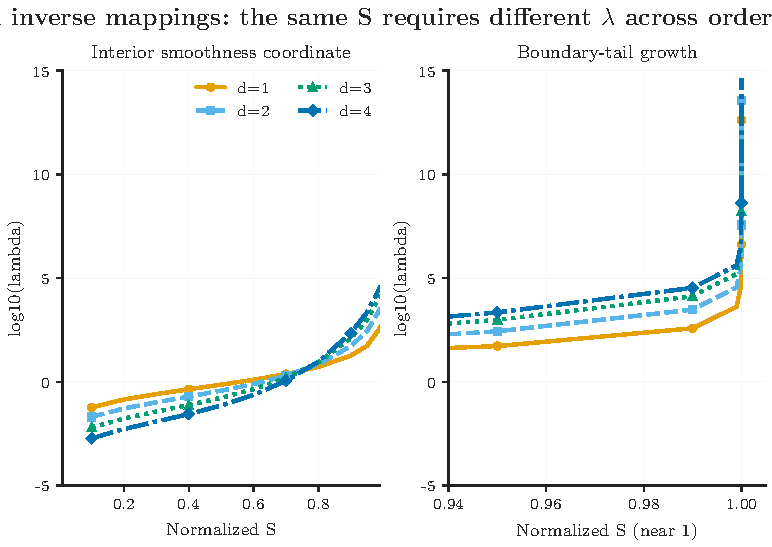
\includegraphics[width=\linewidth]{figures/sncs_smoothness_mapping.pdf}
\caption{Archived $S\mapsto\lambda$ inversions for
$n=24$, $d=1,\ldots,4$. The left panel covers the interior
of the common normalized coordinate; the right enlarges
the high-smoothness tail. A common $S$ need not imply a
common numerical penalty across difference orders.
The exact $S=1$ boundary has $\lambda=\infty$ and is
excluded from logarithmic ordinates.}
\label{fig:expanded-s-mapping}
\end{figure}

\subsection{Numerical inversion in log-penalty coordinates}
For an interior target $s$, numerical inversion solves
$F(x)=S(e^x)-s=0$ in $x=\log\lambda$. Differentiation gives
\begin{equation}
F'(x)=\frac{1}{r}\sum_j
\frac{e^x\delta_j}{(1+e^x\delta_j)^2}.
\label{eq:expanded-log-derivative}
\end{equation}
A bracket ensures that safeguarded Newton, secant,
Brent and bisection methods cannot escape the admissible
positive-penalty domain. In the tail $s\approx1$, evaluate
\[
1-S(\lambda)=\frac1r\sum_j
\frac{1}{1+\lambda\delta_j}
\]
directly rather than subtracting two nearly equal
floating-point numbers. At $s\approx0$, likewise use $S$
itself for the residual. A small residual in $F$ is not
equivalent to a small relative error in $\lambda$ at the
extreme boundaries; the benchmark records the achieved
relative error in the \emph{smaller smoothness tail}.
This inversion is one of the explicit costs of offering
a human-interpretable smoothness interface.

\subsection{Statistical selection is not a change of estimator}
For a fixed reference mean, let $C(\lambda;\mu)$ denote
one of the already established CV, GCV, AICc, BIC
or conditional Gaussian marginal-likelihood scores
\cite{cortes2017smoothness}. For example, classical
leave-one-out CV can be evaluated through
the fixed-$\mu$ smoother diagonal:
\begin{equation}
\operatorname{CV}(\lambda)
=\frac1n\sum_{i=1}^{n}
\left(\frac{y_i-\widehat\tau_i}{1-h_{ii}}\right)^2,
\qquad h_{ii}=(H_\lambda)_{ii};
\label{eq:expanded-cv}
\end{equation}
and GCV is proportional to
$n\|y-\widehat\tau\|_2^2/[n-\nu_\lambda]^2$.
AICc and BIC use the model's conditional EDF in their
information penalties; MLE profiles a Gaussian
variance-component likelihood conditional on the
specified or plug-in reference difference mean.
The criteria have different numerical scales.

Define $\widetilde C(s;\mu)=C(\Lambda_d(s);\mu)$.
As a mathematical change of variables, global minima
agree when the entire domains and boundary conventions
are treated identically:
\begin{equation}
\arg\min_{s\in[0,1]}\widetilde C(s;\mu)
=S\!\left(\arg\min_{\lambda\in[0,\infty]}
C(\lambda;\mu)\right),
\label{eq:expanded-equiv}
\end{equation}
under the appropriate set-valued interpretation.
For an interior differentiable score,
\[
\frac{\mathrm d\widetilde C}{\mathrm ds}
=\frac{C'(\lambda)}{S'(\lambda)}
=\frac{\mathrm dC/\mathrm d\log\lambda}
       {\mathrm dS/\mathrm d\log\lambda}.
\]
Stationary points are therefore not created by the
coordinate change. However, \emph{finite grids} in $s$
and in $\log\lambda$ generally sample different penalties;
a different numerical minimizer can reflect discretization,
not a change in the underlying statistical criterion.
Our experiments explicitly separate these cases.

\paragraph{Reference-mean caveat.}
When fitting, the package permits a fixed numeric $\mu$
or the observed-difference plug-in
$\widehat\mu=\operatorname{mean}(D_dy)$.
The public Gaussian MLE selector permits \texttt{mu="data"};
classical CV/GCV/AICc/BIC require a fixed numeric $\mu$.
For the data-derived comparison, the numeric estimate
is computed from \emph{training data only} and then
held fixed inside the classical criterion.
This is not the exact CV that would refit $\mu$ at every
leave-one-out deletion, nor joint MLE of $(\mu,\lambda)$.
